\documentclass[UTF8,12pt]{ctexart}
%加载包
\usepackage{ctex}
\usepackage{geometry}%排版
%a4版面,页边距1英寸,showframe 增加边框的参数。
% 设置为A4纸,边距适中模式(永中office)
\geometry{%
	width = 210mm,%
	height = 297mm,
	left = 31.8mm,%
	right = 31.8mm,%
	top = 25.4mm,%
	bottom = 25.4mm%
}

%\hyphenpenalty = 1000% 断字设置,值越大,断字越少。
%\setlength{\parindent}{2em}% 缩进
%\setlength{\parskip}{0.5ex} % 段间距

\usepackage{cite} %引用
\usepackage{amsmath}
\usepackage{amsfonts}
\usepackage{amssymb}%公式
\usepackage{amsthm}%定理环境

%\usepackage{ntheorem}%定理环境,使用这个会使\maketitle版式出问题
\usepackage{bm}%加粗

\usepackage{mathrsfs}
\numberwithin{equation}{section}%对公式以节{section}为基础进行编号.变成(1.1.1)有chapter才有1.1.1,不然只有section是1.1
%\theoremstyle{plain}%定理用latex默认的版式
\newtheorem{thm}{Theorem}[section]
%\theoremstyle{definition}%定义用definition格式
\newtheorem{defn}{Definition}
%\theoremstyle{remark}%用remark格式
\newtheorem{lemma}[thm]{lemma}
\newtheorem{example}{Example}[section]

\usepackage{multirow}%表格列合并宏包,\multirow命令.

\usepackage{tabularx}%表格等宽,\begin{tabularx}命令.

 
%盒子
\usepackage[many]{tcolorbox}    	% for COLORED BOXES (tikz and xcolor included)
\usepackage{setspace}               % for LINE SPACING
\usepackage{multicol}               % for MULTICOLUMNS
%自定义设定		
	\definecolor{main}{HTML}{5989cf}    % setting main color to be used
	\definecolor{sub}{HTML}{cde4ff}     % setting sub color to be used
	
	\newtcolorbox{boxF}{
		colback=blue!5!white,
		enhanced,
		boxrule = 1.5pt, 
		colframe = white, % making the base for dash line
		borderline = {1.5pt}{0pt}{main, dashed} % add "dashed" for dashed line
	}
\tcbuselibrary{skins, breakable}% 支持文本框跨页

\usepackage[english]{babel}% 载入美式英语断字模板

\usepackage{graphicx}
\usepackage{float}
\usepackage{subfigure} %插入多图时用子图显示的宏包

\usepackage{algorithm,algorithmic}%算法

\usepackage{listings}   %代码块
\usepackage{xcolor}
\definecolor{codegreen}{rgb}{0,0.6,0}
\definecolor{codegray}{rgb}{0.5,0.5,0.5}
\definecolor{codepurple}{rgb}{0.58,0,0.82}
\definecolor{backcolour}{rgb}{0.95,0.95,0.92}
%设置代码块
\lstdefinestyle{mystyle}{
	backgroundcolor=\color{backcolour},   
	commentstyle=\color{codegreen},
	keywordstyle=\color{magenta},
	numberstyle=\tiny\color{codegray},
	stringstyle=\color{codepurple},
	basicstyle=\ttfamily\footnotesize,
	breakatwhitespace=false,         
	breaklines=true,                 
	captionpos=b,                    
	keepspaces=true,                 
	numbers=left,                    
	numbersep=5pt,                  
	showspaces=false,                
	showstringspaces=false,
	showtabs=false,                  
	tabsize=2
}

\lstset{style=mystyle,
	language=R,                                       % 设置语言
}

\usepackage{appendix}%附录

\usepackage{hyperref}%可以生成pdf书签,可以跳转
\hypersetup{
	colorlinks=true,
	linkcolor=black,
	citecolor=black,
}%使得目录没有红框 参考文献引用没有颜色

%侧栏笔记
\usepackage{marginnote}
\setlength{\marginparwidth}{2.8cm}%设置宽度
\renewcommand*{\marginfont}{\color{violet}\footnotesize}%fonts
%运用此命令就可加入侧栏笔记\normalmarginpar\marginnote{}

%图注
\usepackage{caption}

%参考文献
\usepackage[round]{natbib}


%画图
\usepackage{tikz}
\usetikzlibrary{patterns}
%标题页
\title{Notes of Particle Filter 2022 9}
\author{任何}
\date{ }

%工具
%使用文本框
%\begin{tcolorbox}[enhanced]	\end{tcolorbox}
%代码框
%{\setmainfont{Courier New Bold}                       %设置代码字体                   
%\begin{lstlisting}

%\end{lstlisting}}

%文章开始部分

\begin{document}
	\captionsetup[figure]{labelfont={bf},labelformat={default},labelsep=period,name={图}}%设置图注
	
	\maketitle
	\tableofcontents%目录
	\listoffigures%图片目录
	\listoftables%表格目录
	\newpage
	\kaishu
	
	
	%------------------------------------------- 
	\section{Backgroud}
    对于动态模型(Dynamic Model),主要有以下几类:
    %
    $$
       Dynamic \ model
       \left\{\begin{matrix}
       	HMM,\\
       	Linear \ Dynamic \ system,\\
       	Non-Linear,Non-Gausss.
       \end{matrix}\right.
    $$
	\begin{figure}[H]
		\centering
		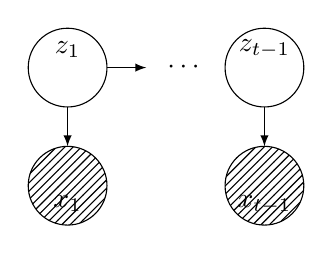
\begin{tikzpicture}[>=latex,scale=0.5]
			\draw (0,0) circle(1)node[above]{$z_1$};
			\draw[pattern=north east lines] (0,-3) circle(1)node[below]{$x_1$};
			\draw[->] (0,-1)--(0,-2);
			\draw[->] (1,0)--(2,0);
			\node at (3,0) {$\cdots$};
			%平移变换
			\draw[xshift=5cm] (0,0) circle(1)node[above]{$z_{t-1}$};
			\draw[pattern=north east lines,xshift=5cm] (0,-3) circle(1)node[below]{$x_{t-1}$};
			\draw[->,xshift=5cm] (0,-1)--(0,-2);

		\end{tikzpicture}
		\caption{Dynamic Model}
	\end{figure}
	%-------------------------------------------
	\newpage
	\begin{appendices}
		\section{R code}

		
	\end{appendices}
	
	%参考文献
	%-------------------------------------------
	\newpage
	%\bibliographystyle{plainnat}%
	%\bibliography{refs.bib}
\end{document}